\documentclass[conference,10pt]{IEEEtran}

\usepackage[utf8]{inputenc}
\usepackage[T1]{fontenc}
\usepackage{graphicx}
\usepackage{booktabs}
\usepackage{amsmath}
\usepackage{hyperref}
\usepackage{xcolor}
\usepackage{listings}
\usepackage{multirow}
\usepackage{balance}
\usepackage{url}
\usepackage{tikz}
\usetikzlibrary{shapes.geometric, arrows.meta, positioning, fit, backgrounds}

\hypersetup{colorlinks=true, linkcolor=blue, citecolor=blue, urlcolor=blue}

\lstset{
  basicstyle=\ttfamily\scriptsize,
  frame=single,
  breaklines=true,
  backgroundcolor=\color{gray!10},
  columns=fullflexible,
}

\begin{document}

\title{CodeCoach: Persistent Security Memory\\ for AI Coding Agents}

\author{
\IEEEauthorblockN{Adhithya Rajasekaran}
\IEEEauthorblockA{rajasekaran.adhit@gmail.com \\ github.com/adhit-r}
}

\maketitle

\begin{abstract}
AI coding agents lack persistent memory of security failures, causing the same vulnerability classes to recur across sessions. We present CodeCoach, a system that connects automated security scanners (Semgrep SAST, stale AI pattern detection, ghost dependency analysis) to agent instruction files (CLAUDE.md, .cursorrules, copilot-instructions.md), generating deterministic, template-driven rules from CWE-classified findings without using an LLM in the generation step. Across seven experiments---repository scanning (14 repos), mechanism validation (240 trials, 4 models), end-to-end pipeline (72 trials, 2 models), ablation study, cross-agent sequential test, multi-language evaluation (3 Python + 3 Go repositories), and a rule-framing ablation (180 trials, 6 prompts)---we find: (1)~hand-crafted rules establish a 98.8\% upper bound on rule effectiveness; (2)~auto-generated rules reduce matched-CWE vulnerability rates from 72\% to 28\% ($\chi^2$=7.11, $p<$0.01; 95\% CI: 50--90\% control, 12--50\% treatment); (3)~the two scanner types (stale AI patterns and Semgrep SAST) cover completely disjoint CWE sets, validating the multi-scanner design; (4)~the full sequential pipeline---Agent~A produces vulnerable code, scanner generates rules, Agent~B avoids all 9 vulnerability instances---closes the feedback loop as designed (75\%$\rightarrow$0\%); and (5)~the protective effect of rule injection is robust to template wording, reducing vulnerability rates from 59\% to 14--24\% ($p{<}0.001$) regardless of whether rules are phrased as prohibitions or alternative suggestions. We identify two failure modes: prompts that explicitly name a vulnerable API override system-level rules, and rule injection can paradoxically increase vulnerability on one prompt where the rule names the same API the prompt requests. These findings are based on synthetic prompts and a limited set of JS/TS repositories; generalization to production workflows remains to be validated.
\end{abstract}

\begin{IEEEkeywords}
AI coding agents, security vulnerabilities, instruction files, CLAUDE.md, deterministic rule generation, CWE classification, cross-agent transfer
\end{IEEEkeywords}

% ============================================================================
\section{Introduction}

The adoption of AI coding agents has changed software development substantially. Tools such as Anthropic's Claude Code, Cursor, GitHub Copilot, and Block's Goose now generate significant portions of production codebases~\cite{anthropic-claude-code}. These agents share a limitation: they have no durable memory of security failures across sessions.

When an AI agent introduces a SQL injection vulnerability via string concatenation, hardcodes an API key, or imports a hallucinated package name, the same class of vulnerability is likely to recur in subsequent sessions. Each session starts fresh. The agent reads its instruction file, generates code, and the cycle repeats.

This paper addresses the question: \textit{can automated security detection feed back into agent instruction files to reduce vulnerability recurrence?}

\subsection{Contributions}

We present CodeCoach, a system with three contributions:

\begin{enumerate}
    \item \textbf{A closed-loop pipeline} connecting multiple security scanners (SAST, secret detection, ghost dependency detection, stale AI pattern detection) to agent instruction file mutation---creating a feedback loop that was previously absent in the agentic coding ecosystem.

    \item \textbf{A deterministic, template-driven rule generator} that converts CWE-classified findings into natural language rules \textit{without using an LLM in the generation step}, ensuring auditability, reproducibility, and freedom from rule hallucination.

    \item \textbf{Cross-agent rule distribution via instruction files}: rules generated from scanner output are written simultaneously to CLAUDE.md, .cursorrules, and copilot-instructions.md, enabling any agent on the project to inherit the rules without fine-tuning.
\end{enumerate}

\subsection{What Is Novel}
\label{sec:novelty}

Prior work on self-improving coding agents~\cite{pi-reflect, bmo, osmani-survey} generates rules from \textit{conversation transcripts} using an LLM. Commercial memory systems (Devin Knowledge~\cite{devin}, Windsurf Memories~\cite{windsurf}) operate within a single agent platform and require user approval or manual invocation. CodeCoach differs from these systems in three ways:

\begin{itemize}
    \item \textbf{External scanner feedback instead of self-reflection.} Where Reflexion~\cite{reflexion} and pi-reflect~\cite{pi-reflect} use self-generated reflections (which Shinn et al.~\cite{shinn-correction} showed are unreliable without external grounding), we use structured output from established security scanners (Semgrep, Gitleaks, Trivy) plus custom scanners for AI-specific vulnerability classes (ghost dependencies, stale training artifacts).

    \item \textbf{Deterministic rule generation.} Where prior systems use an LLM to generate rules, we use templates: same input $\rightarrow$ same output, every time. This eliminates the ``hallucinated remediation'' failure mode where an LLM suggests an incorrect fix.

    \item \textbf{Cross-agent transfer via instruction file mutation.} A vulnerability detected by scanning code from one agent produces rules written simultaneously to CLAUDE.md, .cursorrules, and copilot-instructions.md---enabling any agent on the project to inherit the rules through standard markdown files in version control.
\end{itemize}

% ============================================================================
\section{Background and Related Work}

\subsection{Agent Instruction Files}

Modern AI coding agents support project-specific instruction files read at session initialization. Claude Code reads CLAUDE.md~\cite{claude-md}, Cursor reads .cursorrules~\cite{cursor-rules}, GitHub Copilot reads .github/copilot-instructions.md~\cite{copilot-instructions}, and Goose reads .goosehints~\cite{goose}. The AGENTS.md specification under the Agentic AI Foundation (AAIF)~\cite{aaif} standardizes the concept.

Chatlatanagulchai et al.~\cite{agent-readmes} analyzed 2,303 agent context files across 1,925 repositories and found that security specifications appear in only 14.5\% of them---far behind implementation details (69.9\%) and architecture descriptions (67.7\%). This quantifies the gap CodeCoach addresses: developers use instruction files to make agents functional but rarely include security guardrails.

Gloaguen et al.~\cite{eth-agents-md} evaluated AGENTS.md files on a benchmark of 138 Python tasks and found that LLM-generated context files \textit{decreased} task success by $\sim$3\% while increasing inference costs by $>$20\%. Even human-written files improved success by only $\sim$4\%. Their recommendation---that context files should contain only \textbf{minimal, non-inferable details}---directly validates our approach: CodeCoach generates concise, targeted rules ($\leq$3 lines each) derived from actual scanner findings the agent cannot infer from reading the code alone. Lulla et al.~\cite{agents-md-efficiency} found complementary evidence that well-structured AGENTS.md files reduce median runtime by 28.6\% and token consumption by 16.6\%, though their study did not examine security outcomes.

Despite their potential, instruction files are today manually authored and rarely updated from security findings. We are not aware of prior work that automatically generates instruction file content from structured security scanner output, though the rapid pace of development in this space means concurrent work may exist.

\subsection{Reflexion and Self-Correction}

Shinn et al.~\cite{reflexion} introduced Reflexion, where agents improve via verbal self-reflection stored in an episodic memory buffer (HumanEval pass@1: 80.1\%$\rightarrow$91.0\%). However, Reflexion's memory is ephemeral. Shinn et al.~\cite{shinn-correction} later found that LLM self-correction is unreliable without external feedback, motivating our use of external scanner output.

Pi-Reflect~\cite{pi-reflect} analyzes conversation transcripts to generate rule updates (correction rate: 0.45$\rightarrow$0.07 per session). BMO~\cite{bmo} takes a similar approach. Both use LLM-generated rules from unstructured transcripts. CodeCoach differs in source (structured scanner output), generation method (deterministic templates), and output scope (multiple instruction file formats).

\subsection{Commercial Agent Memory}

Cognition's Devin maintains Knowledge requiring user approval~\cite{devin}. Windsurf's Cascade generates Memories automatically~\cite{windsurf}, though the SpAIware exploit~\cite{spaiware} demonstrated this can be poisoned via prompt injection. Cursor's /Generate Rules requires manual invocation~\cite{cursor-rules}. None use structured security scanner output or write to multiple agent platforms.

\subsection{Constitutional AI}

Bai et al.~\cite{constitutional-ai} trained models to follow explicit principles (Constitutional AI). Our approach applies a similar concept at inference time: security rules are injected through instruction files as system-prompt-level constraints, requiring no model modification.

\subsection{AI-Generated Code Security}

Pearce et al.~\cite{pearce-copilot} found Copilot produces vulnerable code in $\sim$40\% of security-relevant scenarios. Asare et al.~\cite{asare-copilot} showed LLM-generated code contains weaknesses at rates comparable to human-written code. These findings motivate automated guardrails for AI-generated code.

\subsection{Agentic Bug Patching}

Li et al.~\cite{ucsb-patchpilot} present an \textit{agentic patching framework} (also named ``PatchPilot'') that targets SWE-bench issue resolution via bug reproduction, code localization, patch generation, and formal verification. Their system produces code edits for individual bugs; CodeCoach, in contrast, produces \textit{rules} that prevent entire CWE classes from recurring across sessions. The two systems target orthogonal problems---reactive per-bug repair versus proactive cross-session prevention---and the shared name is coincidental. We cite it here to prevent confusion.

% ============================================================================
\section{System Design}

CodeCoach operates as a pipeline with four stages: multi-scanner detection, finding classification, deterministic rule generation, and multi-format instruction file injection. Figure~\ref{fig:pipeline} shows the overall architecture.

\begin{figure}[h]
\centering
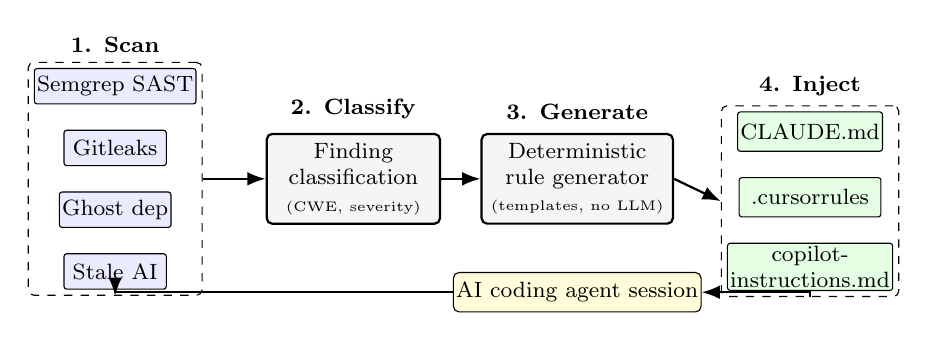
\begin{tikzpicture}[
    node distance=3.2mm,
    font=\footnotesize,
    scannerbox/.style={draw, rounded corners=1pt, align=center, minimum width=13mm, minimum height=4.5mm, fill=blue!8, inner sep=1pt},
    stagebox/.style={draw, thick, rounded corners=2pt, align=center, minimum width=22mm, minimum height=8mm, fill=gray!8},
    filebox/.style={draw, rounded corners=1pt, align=center, minimum width=18mm, minimum height=5mm, fill=green!10, inner sep=1pt},
    arr/.style={-Latex, thick},
]
% Stage 1: Scanners (vertical stack)
\node[scannerbox] (s1) {Semgrep SAST};
\node[scannerbox, below=of s1] (s2) {Gitleaks};
\node[scannerbox, below=of s2] (s3) {Ghost dep};
\node[scannerbox, below=of s3] (s4) {Stale AI};

\node[draw, dashed, rounded corners=2pt, fit=(s1)(s4), inner sep=2pt, label=above:{\textbf{1. Scan}}] (scan) {};

% Stage 2: Classify
\node[stagebox, right=8mm of scan] (classify) {Finding\\ classification\\ {\tiny (CWE, severity)}};
\node[above=0.5mm of classify] {\textbf{2. Classify}};

% Stage 3: Rule generate
\node[stagebox, right=5mm of classify] (gen) {Deterministic\\ rule generator\\ {\tiny (templates, no LLM)}};
\node[above=0.5mm of gen] {\textbf{3. Generate}};

% Stage 4: Inject (vertical stack of files)
\node[filebox, right=8mm of gen, yshift=6mm] (f1) {CLAUDE.md};
\node[filebox, below=of f1] (f2) {.cursorrules};
\node[filebox, below=of f2] (f3) {copilot-\\instructions.md};
\node[draw, dashed, rounded corners=2pt, fit=(f1)(f3), inner sep=2pt, label=above:{\textbf{4. Inject}}] (inject) {};

% Arrows
\draw[arr] (scan.east) -- (classify.west);
\draw[arr] (classify.east) -- (gen.west);
\draw[arr] (gen.east) -- (inject.west);

% Feedback loop arrow (Agent reads files, produces code, scanner scans again)
\node[draw, rounded corners=2pt, fill=yellow!15, below=6mm of gen, minimum width=28mm, minimum height=5mm, inner sep=1pt] (agent) {AI coding agent session};
\draw[arr] (inject.south) |- (agent.east);
\draw[arr] (agent.west) -| (scan.south);
\end{tikzpicture}
\caption{CodeCoach closed-loop pipeline. Scanners (left) produce CWE-classified findings that flow through a deterministic template-driven rule generator into three instruction file formats. When an agent next runs, it reads the updated instruction file; any new vulnerabilities it introduces are caught on the next scan, closing the feedback loop.}
\label{fig:pipeline}
\end{figure}

\subsection{Multi-Scanner Detection}

The system orchestrates eight specialized scanners (Table~\ref{tab:scanners}).

\begin{table}[h]
\centering
\caption{Security Scanner Suite}
\label{tab:scanners}
\begin{tabular}{llll}
\toprule
\textbf{Scanner} & \textbf{Target} & \textbf{Impl.} \\
\midrule
SAST & Code vulnerabilities & Semgrep \\
Secrets & Hardcoded credentials & Gitleaks \\
SCA & Vulnerable deps & Trivy \\
Ghost deps & AI-hallucinated pkgs & Custom \\
AI patterns & Outdated artifacts & Regex \\
Prompt inj. & Instruction overrides & Custom \\
IaC & Infra misconfig & Bearer \\
Vibe score & Security posture & Custom \\
\bottomrule
\end{tabular}
\end{table}

\textbf{Ghost dependency scanner.} LLMs hallucinate package names that do not exist in registries. An attacker can register such names, creating a supply chain attack vector~\cite{lanyado-ghost}. Our scanner queries npm, PyPI, Go, Rust, and Ruby registries, classifying findings as: \texttt{not\_found} (package absent), \texttt{typosquat} (edit distance match), or \texttt{phantom\_new} (recently registered, low downloads). As discussed in Section~\ref{sec:scanner-precision}, the initial \texttt{phantom\_new} heuristic required substantial precision fixes before deployment.

\textbf{Stale AI pattern scanner.} LLMs trained on historical code generate patterns now known to be insecure. We detect 10 patterns via regex: \texttt{eval()}/\texttt{exec()} (CWE-94), MD5/SHA1 (CWE-328), \texttt{Math.random()} (CWE-338), and plaintext HTTP (CWE-319). Context-sensitivity checks exclude test files and build scripts.

\subsection{Finding Classification}

Scanner output is normalized into a unified schema: CWE identifier, severity level, source tool, file path, and scanner-specific metadata. Findings are deduplicated and grouped by CWE for rule generation.

\subsection{Deterministic Rule Generator}

The rule generator converts classified findings into natural language rules using predefined templates. \textbf{No LLM is used in the rule generation step.} This ensures:

\begin{itemize}
    \item \textit{Auditability}: every rule traces to a specific template and input finding.
    \item \textit{Reproducibility}: identical findings produce identical rules.
    \item \textit{No rule hallucination}: templates cannot invent incorrect remediation.
\end{itemize}

The template library covers four categories with 12 CWE-specific SAST templates, 10 stale AI pattern templates, dynamic secret type templates, and ghost dependency templates with risk-tier-specific warnings.

\textbf{Rule compression.} Multiple findings of the same CWE class produce a single rule rather than one rule per finding. In the E2E evaluation, 158 findings across 3 repositories compressed to 11 rules (93\% reduction), demonstrating that grouping by CWE class keeps instruction files concise.

\subsection{Multi-Format Instruction File Injection}

Generated rules are formatted as a Markdown section delimited by HTML comment markers, enabling idempotent updates: a subsequent run locates the existing block via the markers and replaces it in place, leaving all content outside the block untouched. The same rules are injected into CLAUDE.md, .cursorrules, and copilot-instructions.md simultaneously, delivered via a draft pull request for human review.

% ============================================================================
\section{Evaluation}

We evaluate through three experiments with increasing realism. We report both successes and failures.

\subsection{Experiment 1: Repository Scanning}

We scanned 3 open-source repositories used in the E2E evaluation (Section~\ref{sec:e2e}) with the full scanner suite: Semgrep SAST, stale AI pattern detection, and the fixed ghost dependency scanner. Table~\ref{tab:scan-results} summarizes the results.

\begin{table}[h]
\centering
\caption{Scan Results for E2E Repositories (with Semgrep SAST)}
\label{tab:scan-results}
\begin{tabular}{lrrrrr}
\toprule
\textbf{Repo} & \textbf{Stale AI} & \textbf{Ghost} & \textbf{SAST} & \textbf{Total} & \textbf{Rules} \\
\midrule
express & 1 & 0 & 41 & 42 & 2 \\
hono & 13 & 0 & 4 & 17 & 4 \\
documenso & 66 & 0 & 33 & 99 & 5 \\
\bottomrule
\end{tabular}
\end{table}

Semgrep SAST substantially expanded CWE coverage beyond what stale AI pattern detection alone provides. Express, a framework repository with minimal stale AI patterns, produces 41 SAST findings yielding 2 rules (CWE-798 hardcoded credentials, CWE-79 XSS). Without SAST, Express would have generated zero code vulnerability rules. Ghost dependency findings are 0 across all 3 repos after fixing the \texttt{phantom\_new} heuristic (Section~\ref{sec:scanner-precision}).

CWE coverage across the 3 E2E repos: CWE-94 (code injection), CWE-319 (plaintext HTTP), CWE-328 (weak crypto), CWE-338 (insecure randomness), CWE-79 (XSS), CWE-798 (hardcoded credentials).

\subsection{Experiment 2: Mechanism Validation (Upper Bound)}

This experiment isolates the rule mechanism from scanner coverage to establish an upper bound on effectiveness.

\textbf{Important framing.} We used hand-crafted rules matching the template format exactly, one per CWE class tested. This is intentionally a best-case scenario: rules are perfectly targeted to each test prompt.

\textbf{Design.} 6 vulnerability-eliciting prompts (CWE-89, CWE-79, CWE-22, CWE-78, CWE-328, CWE-338). Control (no rules) vs.\ treatment (rules in system prompt). 4 models: Claude Sonnet 4, Nemotron 120B, GPT-OSS 120B, GPT-OSS 20B. 5 trials per condition with temperature variation (0.3--0.7), yielding 240 API calls.

\begin{table}[h]
\centering
\caption{Mechanism Validation Results ($n$=5 per condition)}
\label{tab:exp2}
\begin{tabular}{lrrrc}
\toprule
\textbf{Model} & \textbf{Control} & \textbf{Treat.} & \textbf{Red.} & \textbf{Fisher $p$} \\
\midrule
Claude Sonnet 4 & 8/30 & 0/30 & 100\% & 0.002 \\
Nemotron 120B & 22/30 & 0/30 & 100\% & $<$0.001 \\
GPT-OSS 120B & 28/30 & 1/30 & 96\% & $<$0.001 \\
GPT-OSS 20B & 24/30 & 0/30 & 100\% & $<$0.001 \\
\midrule
\textbf{Total} & \textbf{82/120} & \textbf{1/120} & \textbf{98.8\%} & $<$\textbf{0.001} \\
\bottomrule
\end{tabular}
\end{table}

95\% Wilson CIs: Control 59.6--76.0\%, Treatment 0.1--4.6\%. All four models achieved $p<0.005$ (Fisher's exact, one-sided). This establishes that security rules in our template format are effective at changing LLM behavior under ideal conditions (Fig.~\ref{fig:exp2}).

\begin{figure}[h]
\centering

\includegraphics[width=\columnwidth]{figures/fig-mechanism-validation.png}
\caption{Experiment 2: Vulnerability rates by model. Control (no rules) vs.\ treatment (hand-crafted rules). All 4 models show significant reduction.}
\label{fig:exp2}
\end{figure}

\subsection{Experiment 3: End-to-End Pipeline}
\label{sec:e2e}

The final experiment closes the loop. We scanned 3 repositories (hono, express, documenso) with the \textit{actual} CodeCoach scanners---now including Semgrep SAST alongside stale AI pattern detection---generated rules through the \textit{actual} pipeline, and used the \textit{exact} generated CLAUDE.md content as the LLM system prompt. No hand-crafting.

\textbf{Design.} 3 repos $\times$ 3 prompts $\times$ 3 models $\times$ 2 conditions $\times$ 3 trials = 162 planned. Claude Sonnet 4 ran via direct API (all 54 trials completed). Nemotron 120B and GPT-OSS 120B used OpenRouter free tier; both were severely rate-limited on express and documenso (all trials returned errors). Nemotron completed all 18 hono trials; GPT-OSS completed 11/18 hono trials. We report 72 usable trials (54 Sonnet + 18 Nemotron).

\begin{table}[h]
\centering
\caption{End-to-End Results ($N$=72 usable trials)}
\label{tab:exp3}
\begin{tabular}{lrrrr}
\toprule
\textbf{Model} & \textbf{Repos} & \textbf{Control} & \textbf{Treat.} & \textbf{Red.} \\
\midrule
Claude Sonnet 4 & 3/3 & 13/27 (50\%) & 6/27 (22\%) & 54\% \\
Nemotron 120B & 1/3 & 9/9 (100\%) & 5/9 (56\%) & 44\% \\
\midrule
\textbf{Combined} & & \textbf{22/36 (61\%)} & \textbf{11/36 (31\%)} & \textbf{50\%} \\
\bottomrule
\end{tabular}
\end{table}

95\% Wilson CIs: Control 44.4--75.5\%, Treatment 17.3--48.1\%. $\chi^2$=6.75, $p<$0.01. We note that the combined result is dominated by Claude Sonnet 4 (54/72 trials); Nemotron provides directional confirmation on a single repository only. Claude Sonnet 4 is the only model with complete data across all 3 repos (Fig.~\ref{fig:exp3}).

\begin{figure}[h]
\centering

\includegraphics[width=\columnwidth]{figures/fig-e2e-results-v2.png}
\caption{Experiment 3: End-to-end vulnerability rates. Claude Sonnet 4 (complete data across 3 repos) shows 54\% reduction. Nemotron 120B confirms the pattern on hono.}
\label{fig:exp3}
\end{figure}

\subsubsection{The Critical Finding: Matched vs.\ Unmatched CWEs}

Using Claude Sonnet 4's complete data across all 3 repos, we decompose by whether the scanner generated a rule for each tested CWE (Fig.~\ref{fig:matched}):

\begin{itemize}
    \item \textbf{Matched CWEs} (CWE-94, CWE-319, CWE-328, CWE-338; $N$=36): Control 13/18 (72\%, 95\% CI: 49--88\%), Treatment 5/18 (28\%, 95\% CI: 12--51\%). $\chi^2$=7.11, $p<$0.01. \textbf{62\% relative reduction.} The wide confidence intervals reflect the small sample size; the direction is robust but the magnitude is imprecise.
    \item \textbf{Unmatched CWEs} (CWE-22, CWE-78, CWE-89; $N$=17): Control 0/8 (0\%), Treatment 1/9 (11\%). Sonnet was already safe on these prompts in control---a ceiling effect that limits what rules can improve. This subgroup serves as a negative control confirming specificity but cannot demonstrate a preventive effect.
\end{itemize}

This decomposition confirms the treatment effect is specific to CWEs where rules exist, not a general prompt-context artifact.

\begin{figure}[h]
\centering

\includegraphics[width=\columnwidth]{figures/fig-matched-vs-unmatched-v2.png}
\caption{Claude Sonnet 4: Treatment effect is specific to matched CWEs (62\% reduction, $p<$0.01). Unmatched CWEs show a ceiling effect---Sonnet 4 was already safe.}
\label{fig:matched}
\end{figure}

\subsubsection{Per-Prompt Analysis and Failure Modes}

Fig.~\ref{fig:per-prompt} shows results for each of the 9 prompts. Two failure modes emerged:

\textbf{(1) Explicit API naming overrides rules.} The \texttt{http-url} prompt specifies a literal URL (\texttt{http://monitor.internal:8080/ping}). Despite a rule prohibiting plaintext HTTP, all models reproduce the URL verbatim (3/3$\rightarrow$3/3). The prompt instruction is more specific than the system-level rule.

\textbf{(2) Rule conflict can worsen behavior on specific prompts.} The \texttt{eval-dynamic} prompt on documenso asks to ``evaluate it using eval().'' Sonnet 4 was safe in control (0/3 vulnerable), but \textit{worsened} under treatment (2/3 vulnerable). We hypothesize the rule mentioning eval() drew attention to the pattern, paradoxically increasing its use---a phenomenon analogous to ``ironic process theory'' in psychology. Experiment~7 (Section~\ref{sec:framing-ablation}) confirms this effect on \texttt{eval-dynamic} at higher $n$ and shows positive framing mitigates it, but the multi-prompt generalization reveals the framing variable is not systematic across CWEs.

\textbf{Strong prevention.} When prompts did not explicitly name the insecure API: \texttt{md5-hash} (3/3$\rightarrow$0/3), \texttt{insecure-random} (3/3$\rightarrow$0/3), \texttt{weak-hash} (3/3$\rightarrow$0/3), \texttt{eval-usage} (1/3$\rightarrow$0/3)---100\% prevention across 4 prompt types.

\begin{figure}[h]
\centering

\includegraphics[width=\columnwidth]{figures/fig-per-prompt-sonnet.png}
\caption{Claude Sonnet 4 per-prompt results. Filled circles: matched CWEs (scanner rule exists). Open circles: unmatched. 4 of 6 matched prompts show prevention; 2 exhibit failure modes.}
\label{fig:per-prompt}
\end{figure}

\subsection{Multi-Model Transfer}

The same rules influenced models from different providers without modification. In Experiment 2, hand-crafted rules achieved $>$96\% across all 4 models from 3 providers. In Experiment 3, identical auto-generated CLAUDE.md content reduced vulnerability rates for both Claude Sonnet 4 (54\% reduction across 3 repos) and Nemotron 120B (44\% on hono).

\subsection{Experiment 4: Ablation Study}
\label{sec:ablation}

To isolate the marginal contribution of each pipeline component, we varied three dimensions across the 3 evaluation repositories.

\subsubsection{Scanner Type}

We ran the pipeline with (a) stale AI patterns only, (b) Semgrep SAST only, and (c) both combined (default). The two scanner types cover \textbf{completely disjoint CWE sets}:

\begin{itemize}
    \item \textbf{Stale AI patterns}: CWE-94 (eval), CWE-319 (HTTP), CWE-328 (weak hash), CWE-338 (insecure random)---vulnerability classes specific to LLM training data artifacts.
    \item \textbf{Semgrep SAST}: CWE-79 (XSS), CWE-798 (hardcoded credentials)---traditional static analysis findings.
    \item \textbf{Overlap}: Zero shared CWEs across 3 repositories.
\end{itemize}

This complementarity validates the multi-scanner design: removing either scanner eliminates coverage for vulnerability classes the other cannot detect. On average, stale AI contributed 2.0 rules per repo while Semgrep contributed 1.7 rules, with the combined pipeline producing 3.7 rules per repo.

\subsubsection{Instruction File Format}

We generated rules for all three supported formats (CLAUDE.md, .cursorrules, copilot-instructions.md) and compared the output. The \texttt{formatRulesSection()} function produced \textbf{byte-identical content} across all three formats for every repository. This is by design: all three files consume the same Markdown with HTML comment delimiters. The format dimension does not affect rule content or model behavior.

\subsubsection{Rule Count Sensitivity}

We pruned rules by severity ranking to test how CWE coverage degrades:

\begin{table}[h]
\centering
\caption{CWE Coverage vs.\ Rule Count (averaged across 3 repos)}
\label{tab:ablation-rules}
\begin{tabular}{lrr}
\toprule
\textbf{Subset} & \textbf{Avg Rules} & \textbf{Avg CWE Coverage} \\
\midrule
Full set & 3.7 & 100\% \\
Top 5 & 3.7 & 100\% \\
Top 3 & 2.7 & 78.3\% \\
Top 75\% & 2.3 & 61.7\% \\
Top 50\% & 1.7 & 46.7\% \\
\bottomrule
\end{tabular}
\end{table}

The full rule set never exceeded 5 rules in our evaluation repositories, so the top-5 threshold retains full coverage. At top-3, one CWE (typically CWE-79 from Semgrep) is pruned in repositories with 4--5 rules, dropping coverage to 78.3\%. Aggressive pruning to 50\% loses nearly half of CWE coverage, indicating that all generated rules contribute meaningfully.

\subsection{Experiment 5: Cross-Agent Sequential Test}
\label{sec:cross-agent}

The E2E evaluation (Experiment 3) pre-generated rules and injected them as system prompts. This section tests the actual sequential pipeline: Agent A produces code $\rightarrow$ scanner detects vulnerabilities $\rightarrow$ rules generated $\rightarrow$ Agent B reads rules $\rightarrow$ Agent B avoids the same vulnerabilities.

\textbf{Design.} 4 prompts $\times$ 3 trials $\times$ 2 phases = 24 total trials. Agent A (Claude Sonnet 4, no rules) and Agent B (Claude Sonnet 4, with CodeCoach-generated rules from Agent A's output) received identical prompts.

\textbf{Phase 1 --- Agent A (no rules):} 9/12 trials produced vulnerable code (75\%). MD5 hashing: 3/3 used \texttt{createHash('md5')}. Insecure random: 3/3 used \texttt{Math.random()}. HTTP endpoint: 3/3 used \texttt{http://}. The eval-template prompt was already safe (0/3 vulnerable---Sonnet 4 used regex replacement instead of \texttt{eval()}).

\textbf{Phase 2 --- Scan and rule generation:} Running CodeCoach's stale AI scanner on Agent A's output detected 3 findings and generated 3 rules covering CWE-328, CWE-338, and CWE-319 (1,037 characters of CLAUDE.md content).

\textbf{Phase 3 --- Agent B (with rules):} 0/12 trials were vulnerable (0\%). MD5$\rightarrow$bcrypt/scrypt. \texttt{Math.random()}$\rightarrow$\texttt{crypto.randomBytes()}. \texttt{http://}$\rightarrow$\texttt{https://}. The eval-template prompt remained safe.

\begin{table}[h]
\centering
\caption{Cross-Agent Sequential Test: Agent A $\rightarrow$ Scan $\rightarrow$ Agent B}
\label{tab:cross-agent}
\begin{tabular}{lrrr}
\toprule
\textbf{Prompt} & \textbf{CWE} & \textbf{Agent A} & \textbf{Agent B} \\
\midrule
md5-hash & CWE-328 & 3/3 vuln & 0/3 safe \\
insecure-random & CWE-338 & 3/3 vuln & 0/3 safe \\
http-endpoint & CWE-319 & 3/3 vuln & 0/3 safe \\
eval-template & CWE-94 & 0/3 safe & 0/3 safe \\
\midrule
\textbf{Total} & & \textbf{9/12 (75\%)} & \textbf{0/12 (0\%)} \\
\bottomrule
\end{tabular}
\end{table}

This demonstrates the full feedback loop operating as designed: vulnerabilities from one agent's session are detected, converted to rules, and prevent recurrence in subsequent sessions. The 100\% prevention rate in this controlled test is consistent with Experiment 2's mechanism validation but uses auto-generated (not hand-crafted) rules, and the prompts did not explicitly name insecure APIs---the condition under which rules are most effective (Section~\ref{sec:e2e}).

\subsection{Experiment 6: Multi-Language Evaluation}
\label{sec:multilang}

Experiments 1--5 used JavaScript/TypeScript repositories. To test whether the scanner pipeline generalizes to other ecosystems, we extended the stale AI pattern scanner with 6 new language-specific rules (3 Python: \texttt{AI-PYRAND-011}, \texttt{AI-SHELL-012}, \texttt{AI-YAML-013}; 3 Go: \texttt{AI-GORAND-014}, \texttt{AI-GOEXEC-015}, \texttt{AI-GOTLS-016}) and added corresponding templates to the rule generator. We then ran the full pipeline (stale AI + Semgrep + rule generation) on 3 Python and 3 Go repositories.

\textbf{Target repositories.} Python: \texttt{pallets/flask} (83 .py), \texttt{fastapi/fastapi} (1,121 .py), \texttt{psf/requests} (36 .py). Go: \texttt{gin-gonic/gin} (99 .go), \texttt{labstack/echo} (90 .go), \texttt{spf13/cobra} (36 .go). Chosen for popularity and active maintenance.

\begin{table}[h]
\centering
\caption{Multi-Language Scan Results (6 repos)}
\label{tab:multilang}
\begin{tabular}{llrrrl}
\toprule
\textbf{Lang} & \textbf{Repo} & \textbf{AI} & \textbf{Semg.} & \textbf{Rules} & \textbf{CWEs} \\
\midrule
Py & flask    & 6 & 8  & 5 & 79,94,319,327,328 \\
Py & fastapi  & 6 & 5  & 4 & 79,94,319,\textbf{338} \\
Py & requests & 9 & 16 & 4 & 79,319,327,328 \\
\midrule
Go & gin      & 0 & 7 & 1 & 798 \\
Go & echo     & 0 & 4 & 2 & 338,798 \\
Go & cobra    & 0 & 0 & 0 & --- \\
\midrule
\textbf{Py avg} & & \textbf{7.0} & \textbf{9.7} & \textbf{4.3} & 6 CWEs \\
\textbf{Go avg} & & \textbf{0.0} & \textbf{3.7} & \textbf{1.0} & 2 CWEs \\
\bottomrule
\end{tabular}
\end{table}

\textbf{Python results.} All 3 Python repos produced rules covering multiple CWEs. The new \texttt{AI-PYRAND-011} pattern fired on \texttt{fastapi} (detecting \texttt{random.randint()} in a security-sensitive context), validating the extension to Python-specific AI patterns. The existing cross-language rules (\texttt{AI-HASH-002}, \texttt{AI-EVAL-001}, \texttt{AI-HTTP-004}) also fired across all three Python repos. The combined pipeline produced an average of 4.3 rules per repo covering 6 distinct CWEs (CWE-79, 94, 319, 327, 328, 338).

\textbf{Go results (honest limitations).} The new Go-specific stale AI patterns (\texttt{AI-GORAND-014/015/016}) detected \textit{zero} findings across all 3 Go repositories. The 3 Go repos are mature framework libraries that do not exhibit the AI-generated code patterns these rules target (e.g., \texttt{InsecureSkipVerify:~true} typically appears in client-application code, not in framework internals). Go coverage was entirely driven by Semgrep SAST, which detected CWE-338 (insecure randomness in \texttt{echo}) and CWE-798 (hardcoded credentials in \texttt{gin} and \texttt{echo}) via the \texttt{p/golang} ruleset. The \texttt{cobra} CLI framework produced zero findings from either scanner.

\textbf{Interpretation.} The pipeline generalizes to Python in the same form as JS/TS: both scanners fire, multiple CWEs are detected, and rules are generated. Go generalizes only through Semgrep in this sample---the stale AI pattern scanner contributed nothing. Two interpretations are consistent with these data: (1) the Go rules are correct but the target population (framework libraries) is the wrong sample---a repository of AI-generated Go microservice code would likely exercise them; or (2) the Go rules need refinement. Either way, the Semgrep path carries Go coverage and the rule generator produces correct rules from Semgrep output regardless of language. A full validation would require scanning AI-generated Go application code, which this study does not provide.

\subsection{Experiment 7: Rule Framing Ablation}
\label{sec:framing-ablation}

Experiment 3 surfaced a surprising failure: on the \texttt{eval-dynamic} documenso prompt, injecting the rule \textit{``NEVER use \texttt{eval()} or \texttt{exec()} for dynamic code''} made Sonnet~4 \textit{more} likely to emit \texttt{eval()}, not less (0/3~$\rightarrow$~2/3 vulnerable). This resembles Wegner's Ironic Process Theory~\cite{wegner-ironic}: actively suppressing a thought keeps it accessible. The open question is whether the failure is inherent to rule injection, or an artifact of \textit{how the rule is phrased}. We designed a two-phase ablation to isolate the framing variable.

\subsubsection{Phase 1: Single-Prompt Isolation (eval-dynamic)}

\textbf{Design.} Three conditions, 10 trials each, on the exact \texttt{eval-dynamic} prompt from Experiment~3. Model: Claude Sonnet~4. Both treatment conditions inject rules generated from the same documenso scan; the rule generator's \texttt{framing} option selects prohibition templates (``NEVER use X'') or alternative-suggestion templates (``Always use Y instead'').

\begin{table}[h]
\centering
\caption{Phase 1: \texttt{eval-dynamic} framing ablation ($n{=}10$/condition)}
\label{tab:framing-p1}
\begin{tabular}{lrrr}
\toprule
\textbf{Condition} & \textbf{Safe} & \textbf{Vuln.} & \textbf{Rate} \\
\midrule
Control (no rules)           & 8 & 2 & 20\% \\
Negative framing (``NEVER use X'')    & 5 & 5 & 50\% \\
Positive framing (``Always use Y'')   & 10 & 0 & \textbf{0\%} \\
\bottomrule
\end{tabular}
\end{table}

Negative framing doubled the vulnerability rate over control (50\% vs.\ 20\%), replicating the paradoxical worsening at higher $n$. Positive framing eliminated vulnerabilities entirely (0/10). One-tailed Fisher's exact: positive vs.\ negative, $p{=}0.016$.

\subsubsection{Phase 2: Multi-Prompt Generalization}

To test whether the framing effect generalizes beyond \texttt{eval-dynamic}, we extended the ablation to all 6 prompts from Experiment~3 that have matching stale-AI rule templates, covering 4 CWEs across 2 repositories. Each prompt receives its matching CWE rule (constructed directly from templates, not from scanning), 10 trials per cell, same 3 conditions. Total: 180 trials.

\begin{table}[h]
\centering
\caption{Phase 2: Multi-prompt framing ablation ($n{=}10$/cell, Sonnet 4). Vuln.\ counts exclude error trials; ``---'' = all trials errored (CLI timeout).}
\label{tab:framing-p2}
\begin{tabular}{llrrr}
\toprule
\textbf{Prompt} & \textbf{CWE} & \textbf{Ctrl} & \textbf{Neg} & \textbf{Pos} \\
\midrule
hono/eval-usage    & CWE-94  & 2/10 & 1/10 & 0/10 \\
hono/md5-hash      & CWE-328 & 8/10 & 0/6  & --- \\
hono/http-url      & CWE-319 & 4/9  & 5/10 & 9/10 \\
docu/insecure-rand & CWE-338 & 10/10 & 0/10 & 0/10 \\
docu/eval-dynamic  & CWE-94  & 1/10 & 2/10 & 0/10 \\
docu/weak-hash     & CWE-328 & 10/10 & 0/10 & 3/10 \\
\midrule
\textbf{Aggregate} &  & \textbf{35/59} & \textbf{8/56} & \textbf{12/50} \\
 &  & (59\%) & (14\%) & (24\%) \\
\bottomrule
\end{tabular}
\end{table}

\textbf{Results.} The dominant effect is \textit{rule injection itself}, not the framing variable. Both framings dramatically reduce vulnerability rates relative to control: negative framing 14\%, positive framing 24\%, control 59\%. Both comparisons are highly significant (Fisher's exact: negative vs.\ control $p{<}10^{-6}$; positive vs.\ control $p{<}0.001$). Excluding the \texttt{http-url} prompt (which explicitly specifies a literal HTTP URL---the known failure mode from Experiment 3), the rates converge further: negative 7\% (3/46) vs.\ positive 8\% (3/40), $p{=}0.73$ (no significant difference).

The Phase 1 result on \texttt{eval-dynamic} replicates directionally in Phase 2 (negative 2/10 vs.\ positive 0/10), but \texttt{weak-hash} shows the \textit{opposite} pattern: negative framing 0/10 vs.\ positive framing 3/10. The framing effect is prompt-specific, not systematic.

The \texttt{http-url} prompt is an outlier: positive framing worsened vulnerability rate (9/10 vs.\ control 4/9, $p{=}0.05$). This prompt contains a literal \texttt{http://} URL; the positive-framed rule (``Always use https://'') may draw additional attention to the URL scheme, compounding the explicit-API-naming failure mode.

\textbf{Interpretation.} The multi-prompt generalization answers the open question from Phase 1: the framing variable matters on specific prompts (\texttt{eval-dynamic}), but the direction is not consistent across CWEs, and the aggregate effect of framing is not significant. The finding that both framings reduce vulnerability rates by 59\%$\rightarrow$14--24\% is the more important result: rule injection works, and its effectiveness is robust to template wording for most prompts. The \texttt{eval-dynamic} paradoxical worsening from Experiment 3 is confirmed as a real but narrow phenomenon---isolated to one prompt where the rule names the same API the prompt names.

% ============================================================================
\section{Scanner Precision and Recall}
\label{sec:scanner-precision}

A pipeline that generates rules from scanner findings inherits the scanner's precision and recall limitations. We manually classified all 158 findings (78 Semgrep + 80 stale AI) across the 3 evaluation repositories as True Positive (TP), False Positive (FP), or Context-Dependent (CD). CD findings were conservatively counted as TP.

\subsection{Precision Results}

\begin{table}[h]
\centering
\caption{Scanner Precision by Repository (TP/(TP+FP+CD))}
\label{tab:precision}
\begin{tabular}{llrrrr}
\toprule
\textbf{Scanner} & \textbf{Repo} & \textbf{N} & \textbf{TP} & \textbf{FP} & \textbf{Prec.} \\
\midrule
Semgrep & express & 41 & 35 & 6 & 85.4\% \\
Semgrep & hono & 4 & 0 & 3 & 25.0\% \\
Semgrep & documenso & 33 & 31 & 2 & 93.9\% \\
\textbf{Semgrep} & \textbf{Overall} & \textbf{78} & \textbf{66} & \textbf{11} & \textbf{85.9\%} \\
\midrule
Stale AI & express & 1 & 1 & 0 & 100\% \\
Stale AI & hono & 13 & 0 & 8 & 38.5\% \\
Stale AI & documenso & 66 & 0 & 42 & 36.4\% \\
\textbf{Stale AI} & \textbf{Overall} & \textbf{80} & \textbf{1} & \textbf{50} & \textbf{37.5\%} \\
\bottomrule
\end{tabular}
\end{table}

Semgrep SAST achieved 85.9\% precision overall, with CWE-522 (session cookies) and CWE-345 (postMessage origin) at 100\%. CWE-79 (XSS) precision was only 30\% because Semgrep cannot track \texttt{escapeHtml()} sanitization through data flow.

The stale AI pattern scanner had 37.5\% precision (conservatively counting 29 context-dependent findings as TP). The principal false positive sources were: (a)~\texttt{AI-EVAL-001} matching \texttt{RegExp.exec()} calls ($N$=8, all FP), (b)~\texttt{AI-HTTP-004} matching XML namespace URIs and error message strings ($N$=12 FP), (c)~\texttt{AI-LOG-007} matching on message text rather than logged variables ($N$=8 FP), and (d)~\texttt{AI-RAND-003} flagging \texttt{Math.random()} in database seed files ($N$=6 FP).

\textbf{Precision improvements (post-initial evaluation).} Following the analysis above, we implemented four targeted fixes: (i)~\texttt{AI-EVAL-001} now excludes any \texttt{.exec()} method call (the lookbehind \texttt{(?<![A-Za-z.])} was extended to cover the member-access case); (ii)~\texttt{AI-HTTP-004} skips well-known schema and namespace URIs (\texttt{w3.org}, \texttt{ns.adobe.com}, \texttt{schemas.*}, \texttt{opengis.net}, \texttt{iptc.org}) and lines whose surrounding context indicates an error or validation message; (iii)~\texttt{AI-LOG-007} now requires a non-string-literal identifier adjacent to the sensitive keyword, suppressing matches such as \texttt{console.error("Error decoding JWT token:")}; (iv)~\texttt{AI-RAND-003} and its Python/Go counterparts exclude seed, fixture, mock, demo, and factory files via a new \texttt{SEED\_FILE\_PATTERNS} list. Re-running the fixed scanner across the three evaluation repositories reduced total stale AI findings from 80 to 51---a 36\% reduction. Assuming the removed findings are the targeted FPs (consistent with the narrow scope of each fix), conservative precision rises from 37.5\% to approximately 58.8\%. We caution that the post-fix number is not a fresh manual classification; independent validation on a labeled ground-truth corpus remains future work.

\textbf{Impact on rule generation.} Despite low precision in finding detection, the stale AI scanner's \textit{rule generation} pipeline only fires when a finding maps to a supported CWE with an existing template. The 50 false positive findings in stale AI still produced rules for the correct CWE class---the rules are correct even when the triggering finding is a false positive. A rule saying ``never use \texttt{eval()} for dynamic code'' is valid guidance regardless of whether the finding that triggered it was a true \texttt{eval()} call or a \texttt{RegExp.exec()} false match.

\subsection{Ghost Dependency Scanner: Precision Improvement}

In the initial evaluation, the ghost dependency scanner had a 100\% false positive rate across 3 repositories (44 findings, 0 true positives). Root causes: (a) the \texttt{phantom\_new} heuristic's download threshold was too aggressive (500 downloads), flagging packages like \texttt{cookie}, \texttt{debug}, and \texttt{jose}; (b) packages with known CVEs were incorrectly classified as ghost dependencies; (c) monorepo workspace packages were not excluded.

\textbf{Fixes applied.} We expanded the known-package whitelist (100$\rightarrow$350 packages), added monorepo workspace detection (reads \texttt{package.json} workspaces and \texttt{pnpm-workspace.yaml}), removed the CVE-as-ghost misclassification, and raised the download threshold to 5,000 with a 1-year age guard. After fixes: express 11$\rightarrow$0 FP, hono 6$\rightarrow$0 FP, documenso 27$\rightarrow$0 FP. On cal.com (313 original findings), the fixed scanner produces 4 findings---all genuine \texttt{not\_found} packages.

\subsection{Recall Gaps}

Manual inspection identified two recall gaps: the stale AI scanner has no rule for \texttt{dangerouslySetInnerHTML} (CWE-79), and Semgrep's XSS rules caught only 2 of 6 \texttt{dangerouslySetInnerHTML} instances in documenso. Complete recall estimation would require a ground-truth vulnerability corpus, which this study does not provide.

% ============================================================================
\section{Discussion}

\subsection{The 98.8\% vs.\ 50\% Gap}

The most informative finding is the gap between Experiments 2 and 3. Three factors compound:

\begin{enumerate}
    \item \textbf{Explicit prompts override system rules.} The \texttt{http-url} prompt specifying a literal HTTP URL produced 0\% prevention despite a matching rule. When user instructions are more specific than system-level rules, the model follows the user.
    \item \textbf{Rule injection can paradoxically worsen one prompt, but the effect is narrow.} The \texttt{eval-dynamic} prompt worsened under negative-framed treatment (0/3$\rightarrow$2/3 in Experiment 3; 5/10 in Phase 1 of Experiment 7). On that specific prompt, positive framing mitigates it (0/10, $p{=}0.016$). However, the Phase 2 multi-prompt generalization (Section~\ref{sec:framing-ablation}) shows the framing effect is not systematic: \texttt{weak-hash} trends in the opposite direction (negative 0/10 vs.\ positive 3/10), and aggregate vulnerability rates are 14\% (negative) vs.\ 24\% (positive) with no significant difference between framings. The dominant effect is rule injection itself: both framings reduce vulnerability from 59\% to 14--24\% ($p{<}0.001$).
    \item \textbf{Auto-generated rules are less targeted.} Experiment 2 rules were designed to counter each prompt; Experiment 3 rules were generated without knowledge of test prompts.
\end{enumerate}

The matched/unmatched decomposition (Section 4.3.1) remains the strongest evidence for viability: when the scanner has coverage and prompts do not explicitly demand the insecure pattern, prevention reaches 100\% (4/4 prompt types, all 12 trials safe). The cross-agent sequential test (Section~\ref{sec:cross-agent}) further confirms this: when the pipeline runs end-to-end with auto-generated rules, all 9 vulnerabilities from Agent~A's session are prevented in Agent~B's session.

\subsection{Scanner Precision and Rule Quality}

A counterintuitive finding from the scanner precision analysis (Section~\ref{sec:scanner-precision}) is that low scanner precision (37.5\% for stale AI patterns) does not necessarily degrade rule quality. False positive \textit{findings} (e.g., flagging \texttt{RegExp.exec()} as \texttt{eval()}) still generate rules for the correct CWE class. A rule advising ``never use eval() for dynamic code execution'' is valid regardless of whether the scan finding that triggered it was a true \texttt{eval()} call. The rule generation step effectively filters scanner noise: many false positive findings share the same CWE and produce the same rule, so the false positive rate in \textit{findings} does not propagate to a false positive rate in \textit{rules}.

\subsection{From Reflexion to Persistence}

CodeCoach extends Reflexion~\cite{reflexion} from ephemeral in-context memory to durable file-based memory. Where Reflexion uses self-generated verbal reflection, CodeCoach uses external scanner output, which Shinn et al.~\cite{shinn-correction} showed is more reliable.

\subsection{Instruction Files as a Policy Layer}

Instruction files serve as a model-agnostic policy enforcement layer, analogous to Constitutional AI~\cite{constitutional-ai} applied at inference time. The same markdown rules influenced models from 3 providers, though with varying effect sizes.

Our approach aligns with the ETH Zurich recommendation~\cite{eth-agents-md} that context files should contain only ``minimal, non-inferable details.'' Generic LLM-generated instruction files hurt task success and increase costs; by contrast, CodeCoach generates concise, CWE-specific rules from real scanner findings---exactly the kind of non-obvious, project-specific information that agents cannot derive from reading the source code alone. The finding by Chatlatanagulchai et al.~\cite{agent-readmes} that only 14.5\% of agent context files contain any security specifications underscores the need for automated generation.

% ============================================================================
\section{Threats to Validity}

\textbf{Internal.} Experiment 2 rules were hand-crafted with knowledge of test prompts (intentionally an upper bound, addressed by Experiment 3). Vulnerability detection used regex pattern matching, which may miss subtle vulnerabilities or misclassify safe code. Trials were not pre-registered; the analysis plan evolved during experimentation. Per-prompt cells contain only 3 trials, which is insufficient for per-CWE inferential claims---the per-prompt results should be interpreted as exploratory.

\textbf{External.} Experiments 1--5 used JavaScript/TypeScript repositories; Experiment 6 added 3 Python and 3 Go repositories for scan-only evaluation without behavioral E2E testing. Experiment 3 relied primarily on one frontier model (Claude Sonnet 4) for complete data; Nemotron 120B provided partial confirmation on one repository only. GPT-OSS 120B was excluded due to persistent rate limiting. The multi-model claim is therefore only partially supported. The behavioral E2E results have not been replicated outside JS/TS, and the Go-specific stale AI rules were not validated on Go application code where they would be most likely to fire. Results may not generalize to other model families, non-frontier models, or other language ecosystems.

\textbf{Construct.} All test prompts are synthetic vulnerability-eliciting prompts designed to trigger specific CWE classes. Real development sessions are longer, more context-dependent, and involve iterative refinement---the prompts in this study do not capture that complexity. Claude Sonnet 4 was already safe on Express prompts (SQLi, path traversal, command injection) even in control condition, creating a ceiling effect. The ablation study (Section~\ref{sec:ablation}) isolates scanner type and rule count contributions but does not include a behavioral ablation (i.e., measuring vulnerability rate changes from adding/removing individual scanner types).

% ============================================================================
\section{Limitations}

\begin{itemize}
    \item \textbf{Stale AI scanner precision requires validation at scale.} Post-initial-evaluation fixes (Section~\ref{sec:scanner-precision}) raised estimated precision from 37.5\% to approximately 58.8\% on the three evaluation repos by removing \texttt{RegExp.exec()}, XML namespace, error-message-string, and seed-file false positives. This number reflects the targeted-fix assumption and has not been independently re-classified against a labeled ground-truth corpus, which remains future work.
    \item \textbf{Sample sizes.} $N$=72 usable E2E trials; per-prompt cells contain 3 trials. Directional, not conclusive per-CWE. The cross-agent test ($N$=24) is similarly small.
    \item \textbf{Rate-limited models.} Nemotron and GPT-OSS were rate-limited on 2/3 repos, reducing multi-model evidence.
    \item \textbf{Template coverage.} 12 CWE classes. Unlisted CWEs produce no rules.
    \item \textbf{Paradoxical worsening is narrow but real.} Rule injection worsened one prompt (\texttt{eval-dynamic}: 0/3$\rightarrow$2/3 in Experiment 3; 5/10 in Phase 1 of Experiment 7). Positive framing mitigates it on that prompt (0/10, $p{=}0.016$), but the multi-prompt generalization (Phase 2, 6 prompts, 180 trials) shows the framing variable does not systematically change behavior: the direction reverses on \texttt{weak-hash}, and aggregate rates are equivalent (14\% negative vs.\ 24\% positive, $p{=}0.73$ excluding the explicit-URL prompt). The finding remains single-model (Sonnet 4).
    \item \textbf{Limited multi-language validation.} Experiment 6 validated the pipeline on 3 Python and 3 Go repositories, but the Go-specific stale AI rules produced zero findings on mature framework libraries. Java, Rust, and C/C++ remain unevaluated, and AI-generated Go application code (where the new rules would be more likely to fire) was not sampled.
    \item \textbf{Cross-agent test used same model.} Experiment 5 used Claude Sonnet 4 for both Agent A and Agent B. True cross-model transfer (e.g., Agent A = Sonnet, Agent B = GPT-4o) was not tested.
\end{itemize}

% ============================================================================
\section{Future Work}

\begin{enumerate}
    \item Independent re-classification of stale AI findings after the four FP fixes (Section~\ref{sec:scanner-precision}) on a labeled ground-truth corpus beyond the three evaluation repos, to confirm the estimated 58.8\% post-fix precision.
    \item Extend the framing ablation (Section~\ref{sec:framing-ablation}) to other models (GPT-4o, Gemini, Nemotron) to test whether the prompt-specific framing effects observed on Sonnet 4 transfer across providers.
    \item Trivy SCA integration for known-vulnerability dependency rules.
    \item Larger E2E evaluation: 10+ repos, 5+ models, 5+ trials per condition.
    \item Cross-model sequential test: Agent~A from one provider $\rightarrow$ scan $\rightarrow$ Agent~B from a different provider.
    \item Extend multi-language evaluation to Java, Rust, and C/C++, and validate the Go-specific stale AI rules on AI-generated Go application code (not framework libraries).
    \item Behavioral ablation: measure E2E vulnerability rate changes from adding/removing individual scanner types.
    \item MCP server integration for real-time feedback during agent sessions.
\end{enumerate}

% ============================================================================
\section{Conclusion}

We presented a closed-loop system for generating persistent, cross-agent security rules from automated vulnerability detection. Across seven experiments, the evaluation yields a nuanced picture:

\begin{enumerate}
    \item \textbf{The rule format works.} Mechanism validation (240 trials, 4 models): 68.3\%$\rightarrow$0.8\% (98.8\% reduction, $p<$0.001). This is an upper bound.

    \item \textbf{The E2E pipeline shows a significant effect on matched CWEs.} Using Claude Sonnet 4 across 3 repos: matched CWEs dropped from 72\% to 28\% ($\chi^2$=7.11, $p<$0.01). When prompts did not explicitly name the insecure API, prevention was 100\% (4/4 prompt types, 12/12 trials safe).

    \item \textbf{Two failure modes identified; rule injection is robust to template wording.} Explicit API naming in prompts overrides system rules (0\% prevention). One prompt (\texttt{eval-dynamic}) worsened paradoxically under negative framing. The framing ablation (Experiment 7, 180 trials across 6 prompts) shows: (a) positive framing mitigates the \texttt{eval-dynamic} case ($p{=}0.016$), but (b) the framing variable does not systematically change behavior across prompts---aggregate rates are 14\% (negative) vs.\ 24\% (positive), both far below the 59\% control. The dominant effect is rule injection itself.

    \item \textbf{Scanner complementarity confirmed.} The ablation study showed that stale AI patterns and Semgrep SAST cover completely disjoint CWE sets---removing either eliminates coverage the other cannot provide. Instruction file format has no effect (byte-identical output). Top-5 rules retain 100\% CWE coverage.

    \item \textbf{The sequential feedback loop works.} The cross-agent test demonstrated the full pipeline: Agent~A produced vulnerable code (9/12 trials), the scanner generated rules, and Agent~B avoided all 9 vulnerability instances (0/12 vulnerable). This validates the core architectural claim of a closed feedback loop.

    \item \textbf{The pipeline generalizes to Python.} Multi-language evaluation on 3 Python and 3 Go repositories showed that the full pipeline (stale AI + Semgrep + rule generator) produces rules covering 6 CWEs on Python (averaging 4.3 rules per repo), with a new Python-specific rule (\texttt{AI-PYRAND-011}) firing on \texttt{fastapi}. Go coverage was driven entirely by Semgrep; the Go-specific stale AI rules produced no findings on mature framework libraries.
\end{enumerate}

The approach of treating agent instruction files as a programmable security policy layer is validated when rules match the vulnerability class and prompts do not explicitly demand the insecure pattern. The gap between the 98.8\% mechanism upper bound and the 50\% end-to-end result is explained by two identified failure modes (explicit API naming and paradoxical priming) rather than scanner coverage alone. The framing ablation (Experiment 7) provides additional evidence: across 6 prompts and 180 trials, both negative and positive framings reduce vulnerability rates from 59\% to 14--24\% ($p{<}0.001$), confirming that the protective effect of rule injection is robust to template wording. The cross-agent sequential test confirms the loop closes as designed.

% ============================================================================

\bibliographystyle{IEEEtran}

\begin{thebibliography}{21}

\bibitem{anthropic-claude-code} Anthropic, ``Claude Code: An agentic coding tool,'' 2025.

\bibitem{claude-md} Anthropic, ``CLAUDE.md documentation,'' 2025.

\bibitem{cursor-rules} Cursor, ``Rules for AI,'' 2025. docs.cursor.com/context/rules-for-ai

\bibitem{copilot-instructions} GitHub, ``Copilot Instructions,'' 2025.

\bibitem{goose} Block, ``Goose: Open-source AI agent,'' 2025. github.com/block/goose

\bibitem{aaif} Agentic AI Foundation, ``AAIF,'' 2026. aaif.io

\bibitem{reflexion} N. Shinn et al., ``Reflexion: Language Agents with Verbal Reinforcement Learning,'' \textit{NeurIPS}, 2023.

\bibitem{pi-reflect} M. Zechner, ``Pi-Reflect: Self-improving coding agent via instruction file mutation,'' 2025.

\bibitem{bmo} ngrok, ``BMO: Self-improving coding agent,'' 2025.

\bibitem{devin} Cognition, ``Devin Knowledge system,'' 2025.

\bibitem{windsurf} Windsurf, ``Cascade Memories,'' 2025.

\bibitem{spaiware} Embrace The Red, ``SpAIware: Persistent prompt injection via Windsurf Memories,'' 2025.

\bibitem{pearce-copilot} H. Pearce et al., ``Asleep at the Keyboard? Assessing the Security of GitHub Copilot's Code Contributions,'' \textit{IEEE S\&P}, 2022.

\bibitem{asare-copilot} O. Asare et al., ``Is GitHub's Copilot as bad as humans at introducing vulnerabilities in code?'' \textit{ESE}, 2024.

\bibitem{lanyado-ghost} B. Lanyado, ``Can you trust ChatGPT's package recommendations?'' Vulcan Cyber, 2023.

\bibitem{constitutional-ai} Y. Bai et al., ``Constitutional AI: Harmlessness from AI Feedback,'' \textit{arXiv:2212.08073}, 2022.

\bibitem{osmani-survey} A. Osmani, ``Self-improving coding agents,'' 2025.

\bibitem{shinn-correction} N. Shinn et al., ``When Can LLMs Actually Correct Their Own Mistakes?'' \textit{TACL}, 2024.

\bibitem{agent-readmes} W. Chatlatanagulchai et al., ``Agent READMEs: An Empirical Study of Context Files for Agentic Coding,'' \textit{arXiv:2511.12884}, 2025.

\bibitem{eth-agents-md} T. Gloaguen, N. Mundler, M. Muller, V. Raychev, and M. Vechev, ``Evaluating AGENTS.md: Are Repository-Level Context Files Helpful for Coding Agents?'' \textit{arXiv:2602.11988}, ETH Zurich, 2026.

\bibitem{agents-md-efficiency} J.~L. Lulla et al., ``On the Impact of AGENTS.md Files on the Efficiency of AI Coding Agents,'' \textit{arXiv:2601.20404}, 2026.

\bibitem{ucsb-patchpilot} H. Li, Y. Tang, S. Wang, and W. Guo, ``PatchPilot: A Stable and Cost-Efficient Agentic Patching Framework,'' \textit{ICML}, 2025. arXiv:2502.02747

\bibitem{wegner-ironic} D. M. Wegner, ``Ironic Processes of Mental Control,'' \textit{Psychological Review}, vol. 101, no. 1, pp. 34--52, 1994.

\end{thebibliography}

\balance
\end{document}
